\chapter{Desarrollo}
\label{capitulo3}
\setchapter{Capítulo 3. \emph{Desarrollo}}


El diseño y desarrollo de la extensión al compilador de Graciela fueron llevados
a cabo entre marzo y noviembre del año 2016. Luego de una primera etapa de
revisión del trabajo previo, el proyecto se orientó en seis áreas, a saber,
(1) Manejo de apuntadores, (2) Teoría de Conjuntos, (3) Tipos de dato definidos
por el programador, (4) Tipos Algebraicos Libres, (5) Herramientas para el
programador, (6) Colección de casos de prueba.

% El diseño y desarrollo de la extensión al compilador de Graciela fueron llevados
% a cabo en tres etapas, entre marzo y noviembre del año 2016. En la primera
% etapa,
%#  se estudió el estado del compilador elaborado por Araujo y Jiménez,
%#  se evaluaron las recomendaciones que sobre la semántica de este lenguaje hizo el
%# jurado de este primer proyecto,
%  se revisó la bibliografía relacionada con el manejo de tipos definidos por el
% usuario en el contexto de programación formal,
%  se investigó sobre posibles estructuras de datos para implantar tipos que modelen la teoría de conjuntos,
%  se especificó formalmente la sintaxis para las nuevas funcionalidades propuestas
% y
%  se extendieron los analizadores lexicográfico y sintáctico para concordar con
% dicha especificación formal.
%
% En la segunda etapa,
%  se completó la verificación de tipos en presencia de tipos definidos por el
% usuario y tipos que modelan la teoría de conjuntos,
%  se extendió la biblioteca
% externa de Graciela para soportar expresiones de tipos que modelan la teoría de
% conjuntos,
%  se inició la extensión al generador de código intermedio LLVM para producir las
% instrucciones correspondientes a las nuevas funcionalidades y
%  se escribió una colección de programas que ejercitan las capacidades del
% lenguaje, tanto nuevas como originales, a fin de evaluar que el código generado
% fuera correcto.
%
% En la tercera etapa,
%  se culminó la extensión al generador de código intermedio iniciada en la etapa
% anterior,
%  se extendió el manual de usuario para presentar las nuevas funcionalidades del
% lenguaje,
%  se investigaron formas para permitir que programadores noveles instalen el compilador
% sin mayor dificultad
%  se estudiaron las herramientas necesarias para incorporar facilidades de
% depuración (\emph{debugging}) y análisis de rendimiento (\emph{profiling}) al
% compilador.

%%%%%%%%%%%%%%%%%%%%%%%%%%%%%%%%%%%%%%%%%%%%%%%%%%%%%%%%%%%%%%%%%%%%%%%%%%%%%%%%
%% REVISIÓN DEL TRABAJO PREVIO %%%%%%%%%%%%%%%%%%%%%%%%%%%%%%%%%%%%%%%%%%%%%%%%%
%%%%%%%%%%%%%%%%%%%%%%%%%%%%%%%%%%%%%%%%%%%%%%%%%%%%%%%%%%%%%%%%%%%%%%%%%%%%%%%%
\setcounter{section}{-1}
\section{Revisión del trabajo previo}

En la primera etapa de este proyecto, se estudió el estado del compilador
elaborado por Araujo y Jiménez y se evaluaron las recomendaciones hechas por los
mismos sobre posibles extensiones al lenguaje y al compilador.

Se observó que existían aspectos del compilador que podían ser mejorados, y que
además estas mejoras facilitarían el desarrollo de los objetivos del proyecto,
por lo cual se decidió hacer los cambios que se mencionan en esta sección.

%%%%%%%%%%%%%%%%%%%%%%%%%%%%%%%%%%%%%%%%%%%%%%%%%%%%%%%%%%%%%%%%%%%%%%%%%%%%%%%%
\subsection{Recomendaciones de Araujo y Jiménez en su proyecto de grado}

Como parte de su Proyecto de Grado, Araujo y Jiménez dejaron tres
recomendaciones sobre áreas en las cuales el lenguaje Graciela y su compilador
podían ser extendidos. Estas recomendaciones eran las siguientes:

\begin{itemize}

  \item Ofrecer al programador la posibilidad de crear estructuras de datos
  propias, mediante la implementación de Tipos de Dato Abstractos (TDAs).

  \item Incluir la manipulación de apuntadores por parte del programador,
  ampliando el sistema de tipos del lenguaje Graciela para introducir el tipo
  \textbf{apuntador}. Esta característica sería valiosa principalmente para los
  estudiantes del curso Laboratorio de Algoritmos II, por la importancia de los
  apuntadores en el curso.

  \item Proveer la capacidad de creación de tipos de dato enumerados definidos
  por el programador, con la posibilidad de integrarlos al sistema de operadores
  aritméticos y relacionales del lenguaje.

\end{itemize}

Se decidió tomar la primeras de estas recomendaciones, por su importancia para
los cursos teóricos y prácticos de Algoritmos, ya que una buena parte del
material estudiado en dichos cursos se trata del manejo correcto de estructuras
de datos y aserciones sobre sus comportamientos. Además, como gran parte de
estas estructuras hacen uso de apuntadores por distintas razones, también se
tomó la segunda de las recomendaciones.

No se decidió implementar la extensión de la tercera recomendación puesto que su
aporte a los cursos en los que podría usarse el lenguaje Graciela se consideró
limitado, aunque en definitiva se trata de una extensión valiosa para el
lenguaje en general y se mantiene la recomendación para futuros proyectos de
extensión del lenguaje y su compilador.

%%%%%%%%%%%%%%%%%%%%%%%%%%%%%%%%%%%%%%%%%%%%%%%%%%%%%%%%%%%%%%%%%%%%%%%%%%%%%%%%
\subsection{Modularización de la base de código}

La base de código que recibimos, en la forma de un repositorio \emph{git},
consistía de unos veinticinco archivos escritos en \emph{Haskell} organizados en
un solo directorio. No existía entre estos archivos gran separación de
responsabilidades y varios de ellos contenían código para acciones que no
guardaban relación entre ellas. En particular, se encontró que el Árbol
Sintáctico Abstracto (\textsc{ASA}) estaba representado como un solo tipo de
datos con más de cuarenta constructores distintos.

Así, se decidió separar el código fuente del compilador en cuatro áreas:
\begin{itemize}

  \item Estructuras de datos para representar el \textsc{ASA} de un programa
  escrito en Graciela. Almacenado en el directorio \texttt{AST}, por las siglas
  en inglés para \textsc{ASA} (\emph{Abstract Syntax Tree}).

  \item Análisis sintáctico para convertir un archivo de código Graciela en un
  ASA, verificando simultáneamente su corrección. Almacenado en el directorio
  \texttt{Parser}, por el término en inglés para analizador sintáctico.

  \item Generación de código intermedio LLVM para programas escritos
  correctamente en Graciela que ya han sido convertidos en un ASA. Almacenado en el
  directorio \texttt{LLVM}.

  \item Código que se usa en más de una de las áreas anteriores, como la Tabla
  de Símbolos del compilador y las estructuras de datos para la emisión de
  mensajes de error, y el archivo principal del compilador. Almacenado en el
  directorio raíz del código fuente.

\end{itemize}

En cada una de las primeras tres áreas, se separaron a su vez los procedimientos
y estructuras según la parte del lenguaje Graciela que se estuviera tratando.
Así, el archivo \texttt{AST/Expression.hs} contiene las estructuras de datos
para representar únicamente las expresiones del lenguaje Graciela como un
\textsc{ASA}, mientras que \texttt{Parser/Expression.hs} contiene la lógica del
analizador sintáctico para interpretar y verificar la corrección de las
expresiones, y \texttt{LLVM/Expression.hs} contiene las reglas de traducción de
\textsc{ASA} a código intermedio \textsc{LLVM} para expresiones.

%%%%%%%%%%%%%%%%%%%%%%%%%%%%%%%%%%%%%%%%%%%%%%%%%%%%%%%%%%%%%%%%%%%%%%%%%%%%%%%%
\subsection{Recuperación de errores en análisis sintáctico}

También se observó que, enfrentado a archivos Graciela con errores sintácticos,
el compilador producía errores difíciles de interpretar. Si bien no es sencillo
generar mensajes de error y continuar el proceso de análisis sintáctico para
archivos que no pertenecen a la gramática del compilador, esta es una
característica que se espera de cualquier compilador si se desea popularizar su
uso.

Desafortunadamente, la biblioteca de análisis sintáctico con la que había sido
desarrollado el proyecto, \texttt{Parsec}, no está diseñada para ofrecer
recuperación de errores, de modo que cualquier solución que usara esta
biblioteca tendría problemas en este aspecto, o al menos resultaría compleja y
más propensa a defectos de programación.

Así, se investigaron bibliotecas alternativas para análisis sintáctico y se
consiguió \texttt{Megaparsec}. Como se explica en el Marco Tecnológico,
\texttt{Megaparsec} provee el combinador \texttt{withRecovery}, que permite
agregar recuperación de errores con la técnica de \textit{Panic Mode} (<<modo
pánico>>)~\cite{aho2} a un analizador sintáctico de manera sencilla. Este
combinador recibe una función de recuperación y un analizador sintáctico base, y
ejecuta la primera cuando dicho analizador falla. Por ejemplo, para agregar
recuperación de errores a las instrucciones, separadas por punto y coma, se usó
código como el del fragmento~\ref{lst:withrec}, de modo que, con ligeros cambios
según el contexto del analizador, fue posible agregar recuperación de errores al
compilador.

\begin{haskellcode}[caption=Uso de \texttt{withRecovery}, label=lst:withrec]
withRecovery recover instruction
  where
    recover err = void anyToken `manyTill` match TokSemicolon
               >> tell err
\end{haskellcode}

Otra ventaja de la biblioteca \texttt{Megaparsec} sobre \texttt{Parsec} es que
el \emph{Monad} provisto por la primera, a diferencia del provisto por la
segunda, puede ser utilizado \emph{dentro} de Transformadores de \emph{Monad}s,
permitiendo acumular distintos efectos en una pila de \emph{Monad}s. La utilidad
de esto quedará más clara en la subsección sobre Cuantificaciones.

Finalmente, por tratarse de una bifurcación (\emph{fork}, en inglés) de la
biblioteca \texttt{Parsec}, la mayoría de sus combinadores son idénticos o muy
similares a los de dicha biblioteca, lo cual permitió que la migración del
código de una biblioteca a la otra fuera muy simple.

%%%%%%%%%%%%%%%%%%%%%%%%%%%%%%%%%%%%%%%%%%%%%%%%%%%%%%%%%%%%%%%%%%%%%%%%%%%%%%%%
\subsection{Consideraciones sobre arreglos}

Durante la revisión del compilador original, se consiguió que, como en la
mayoría de los lenguajes de bajo nivel, no se ofrecía verificación de acceso a
arreglos dentro de los límites de los mismos. A pesar de que implantar este tipo
de verificaciones no formara parte explícita de los objetivos del proyecto, se
consideró que podría agregarse esta funcionalidad para mejorar la experiencia
del programador novel.

También se consideró que sería cómodo para el programador poder hablar de
arreglos multidimensionales en lugar de arreglos de arreglos, y así recibir
errores apropiados, a tiempo de compilación, al usar un arreglo de \ingra{n}
dimensiones con un número de índices distinto de \ingra{n}. Por ejemplo,
intentar compilar el fragmento de código~\ref{lst:badarr} emitiría un mensaje de
error acerca del uso de un índice de dimensión 1 para leer de un arreglo de 2
dimensiones. En la versión original del compilador, la situación equivalente
produciría un error acerca de intentar imprimir un objeto de tipo arreglo de
entero, que no expresa el verdadero problema del caso.

\begin{gracielacode}[caption=Error en dimensiones de arreglo, label=lst:badarr]
|[ var arr : array [5, 10] of int
 ;  writeln(arr[3])
]|
\end{gracielacode}

Para evitarle confusión a los programadores, se eliminó la posibilidad de
declarar arreglos de arreglos, y se emite un error a tiempo de compilación
cuando esto se hace, sugiriendo en cambio utilizar arreglos multidimensionales.

Para implementar estos cambios, fue necesario cambiar la representación interna
de los arreglos. Originalmente, funcionaban como los arreglos del lenguaje C; es
decir, declarar un arreglo \ingra{x} de tamaño \ingra{tam} de elementos de
tipo \ingra{T}, era equivalente a reservar un espacio en la pila de tamaño
$\texttt{sizeof(T)} * \texttt{tam}$ y asociarle al identificador \ingra{x} el
apuntador al primer elemento. Los arreglos multidimensionales se escribían como
arreglos de arreglos, e internamente ocupaban un espacio contiguo de memoria.
Como se deseaba almacenar los tamaños de los arreglos junto con sus elementos,
se decidió usar una representación interna de \textit{Dope Vectors}, es decir, una estructura cuya primera entrada es la cantidad de
elementos y cuya segunda entrada es el bloque de memoria donde se almacenan los
elementos.

Específicamente, como se muestra en la figura \ref{fig:diag}, para arreglos de \ingra{n} dimensiones, se generan estructuras
<<cabecera>> de \ingra{n+1} campos, donde los primeros \ingra{n}, de tipo entero
de 32 bit, corresponden a los tamaños en cada dimensión del arreglo ($d_0..d_n$ en la figura), y el último
corresponde a un apuntador a un espacio de memoria contiguo de tamaño
$\texttt{sizeof(T)} * \prod\limits_{i=1}^\texttt{n} dimensi\acute{o}n_i$, que se
reserva en el mismo tipo de memoria que la <<cabecera>>, es decir, en la pila si
es un arreglo estático, o en la memoria dinámica si se trata de un apuntador a
un arreglo inicializado con la instrucción \ingra{new(*)}.

\begin{figure}[h!]
  \hspace{8mm}
  \caption{Representación interna de los arreglos en Graciela.}
  \centering
    \fboxsep=5mm
    \fboxrule=0.75pt
    \fcolorbox{gray}{white}{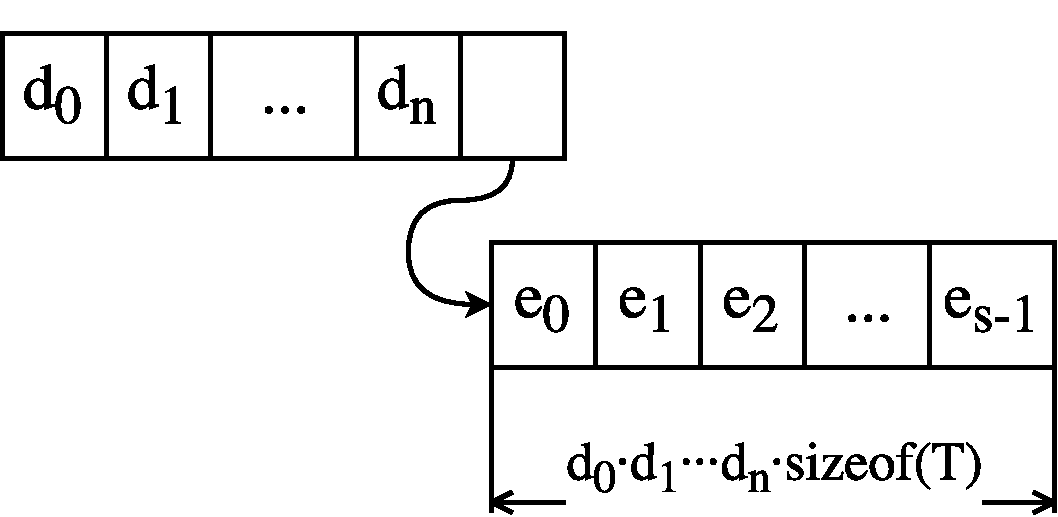
\includegraphics[width=0.5\textwidth]{diag2}}
    \label{fig:diag}
\end{figure}

Cuando todas las dimensiones del arreglo son conocidas a tiempo de compilación,
los tamaños de cada dimensión son almacenados estáticamente en la <<cabecera>> y
se reserva el espacio para los elementos en el tipo de memoria apropiado. Cuando
este no es el caso, se genera el código para, a tiempo de ejecución, evaluar la
expresión correspondiente a cada dimensión del arreglo, almacenar en el campo
correspondiente de la cabecera el valor resultante, y reservar el espacio para
los elementos en el tipo de memoria apropiado.

El hecho de que sean almacenados en dos partes podría causar preocupaciones
respecto a la liberación de memoria ocupada por arreglos dinámicos. Sin embargo,
este caso fue tomado en cuenta y la liberación de memoria procede en dos partes,
liberando primero el bloque de elementos, y posteriormente la <<cabecera>>.

La última consideración sobre los arreglos está asociada con su uso como
parámetros de subrutinas (procedimientos y funciones). Se agregó al lenguaje la
capacidad para usar arreglos como parámetros de los modos In, In-Out y Out,
además del modo Ref ya provisto en la especificación original. Adicionalmente,
se decidió permitir el pase de arreglos de tamaño arbitrario como parámetros
siempre que todas las variables en las expresiones que denotan su tamaño sean
parámetros anteriores de la subrutina, pasados en modo \ingra{const} en el caso
de los procedimientos. Por ejemplo, la firma de procedimiento en el fragmento de código~\ref{lst:arrproc} sería
aceptada por el compilador:

\begin{gracielacode}[caption=Firma de procedimiento con parámetro de tipo arreglo, label=lst:arrproc]
proc sub(
  const size : int,
  inout arr : array [size, size * 2] of int
)
\end{gracielacode}

Desafortunadamente, un procedimiento (o una función) con una firma similar a la
de \ingra{sub} podría ser llamado con argumentos que no concuerden, como en el
fragmento de código~\ref{lst:arrproccall}.

\begin{gracielacode}[caption=Llamada a procedimiento con argumento de tipo arreglo, label=lst:arrproccall]
|[ var arr : array [5, 5]
 ; sub (5, arr)
]|
\end{gracielacode}

En este caso, el procedimiento \ingra{sub} espera un arreglo de tamaño
\ingra{[size, (size * 2)]}, y como recibe \ingra{size = 5}, espera que el tamaño
del arreglo sea \ingra{[5, 1~~0]}. Sin embargo, recibe un arreglo de tamaño
\ingra{[5, 5]}, por lo cual la ejecución debe abortar al momento de esa llamada.
Esta verificación no puede hacerse a tiempo de compilación en el caso general,
puesto que sería equivalente a predecir todos los posibles cursos de ejecución
del programa.

%%%%%%%%%%%%%%%%%%%%%%%%%%%%%%%%%%%%%%%%%%%%%%%%%%%%%%%%%%%%%%%%%%%%%%%%%%%%%%%%
\subsection{Consideraciones sobre funciones y procedimientos}

Se decidió cambiar ligeramente la gramática de las funciones y procedimientos
para que fueran más similares a sus equivalentes en GCL. Simplemente, se
eliminaron los lexemas \ingra{begin} y \ingra{end}, antes usados para
delimitar el procedimiento, y el lexema \ingra{:} entre el identificador de la
subrutina y su lista de parámetros, y se movió la postcondición junto a la
precondición, antes del cuerpo de la subrutina.

Además, se agregó la posibilidad de especificar cotas para las subrutinas luego
de la postcondición y antes del cuerpo, como requisito para hacer llamadas
recursivas dentro de la misma. Así, es un error a tiempo de compilación escribir
una llamada recursiva de una subrutina sin cota. En el caso contrario, el de una
subrutina con cota pero sin recursión, ésta simplemente es ignorada. A pesar de
que esto no estaba dentro de los objetivos de este proyecto, se consideró de
suma importancia, puesto que la recursión sin cotas es equivalente a la
iteración sin cotas, prohibida en el caso de la instrucción \ingra{do .. od}.

El código intermedio LLVM generado para una subrutina recursiva, necesariamente
con cota, además de incluir el cuerpo especificado por el programador, incluye
verificaciones para el decrecimiento y la no-negatividad de la cota. Esto se
logra pasando dos parámetros adicionales a las subrutinas recursivas. El
primero, de tipo booleano, indica si la llamada en curso es la primera llamada a
la subrutina o si se trata de una llamada recursiva. En ambos casos, al entrar a
la subrutina se calcula el valor de la cota, y si es negativa se da un error y
el programa aborta. En caso contrario, si se trata de la primera llamada a la
subrutina, se ejecuta el cuerpo de ésta, pero si se trata de una llamada
recursiva, se compara la cota actual con la anterior, recibida como el segundo
parámetro implícito. Si no hubo decremento en la cota, también se da un error y
el programa aborta. En caso contrario, se ejecuta el cuerpo de la subrutina.

Por último, cabe mencionar que se cambió la semántica del modo de parámetros
\ingra{in}, de forma que los parámetros declarados con este modo pueden ser
reasignados dentro del cuerpo del procedimiento sin afectar el valor del
argumento usado en el punto de llamada. Originalmente, los parámetros de modo
\ingra{in} no podían ser reasignados, pero se consideró que sería conveniente
poder reasignarlos para ofrecer la posibilidad de usar parámetros por su valor
pero aprovechando su espacio en memoria. El comportamiento asociado
anteriormente al modo \ingra{in} ahora corresponde al modo de parámetros
\ingra{const}.

%%%%%%%%%%%%%%%%%%%%%%%%%%%%%%%%%%%%%%%%%%%%%%%%%%%%%%%%%%%%%%%%%%%%%%%%%%%%%%%%
\subsection{Consideraciones sobre cuantificaciones}

Durante el análisis del compilador original, se conoció que las cuantificaciones
presentaban limitaciones en la expresividad de sus rangos. El analizador
sintáctico de esta parte del lenguaje esperaba, específicamente, dos
comparaciones aritméticas, separadas por un operador de conjunción
(\ingra{/\}), seguidas por un lexema <<barra vertical>>
(\ingra{|}). Esto impedía expresar condiciones lógicas distintas de
comparaciones aritméticas, como predicados definidos por el programador, o
incluso condiciones con más de dos comparaciones aritméticas.

Para solucionar esto, se agregó un estado al analizador sintáctico de las
expresiones, usando el \emph{Monad Transformer} \ingra{StateT} sobre el
\emph{Monad} \ingra{Parsec}. En este estado, se guarda información sobre la
pila de variables generadora presentes en un momento dado (la pila vacía en el
caso de las expresiones sin cuantificaciones). Además, se permitió que el
analizador sintáctico de las expresiones devolviera, además de la expresión
conseguida, el rango asociado a ella. Por ejemplo, con la variable generadora
\ingra{x}, la expresión \ingra{x >= 5} tiene asociado el rango $[5, \infty)$.

Cuando el analizador sintáctico se encuentra en una cuantificación, agrega la
variable generadora correspondiente a la pila del estado, e intenta construir un
rango. Los únicos operadores que construyen rangos son la igualdad (\ingra{==}),
que construye rangos <<unitarios>>; las comparaciones aritméticas (\ingra{>},
\ingra{>=}, \ingra{<}, \ingra{<=}), que construyen rangos <<aritméticos>>; y el
operador <<pertenece>> de la Teoría de Conjuntos ($\in$) [ver sección
\ref{sect:sets}], que produce rangos <<conjunto>>, mientras que la constante
booleana \ingra{false} produce el rango <<vacío>>.

Además, el operador de conjunción (\ingra{/\}) devuelve, si es
posible, el rango que resulta de intersectar los rangos asociados a cada uno de
sus operandos. A diferencia de las cuantificaciones lógicas, sin embargo, no se
consideran los rangos generados por el operador de disyunción
(\ingra{\/}), por lo cual si se desea que un rango sea procesado
como tal, debe estar escrito en Forma Normal Conjuntiva. Esto no le resta
expresividad al lenguaje, ya que pueden conseguirse expresiones equivalentes con
el uso de teoremas lógicos, convirtiendo una cuantificación en la disyunción de
varias, o usando el operador de unión de conjuntos (\ingra{~\Union~}).

Finalmente, si se ha construido un rango válido, este se registra en el ASA
correspondiente a la cuantificación. Si el rango es <<aritmético>>, se exige que
existan límites superior e inferior, emitiéndose el error apropiado en caso de
faltar uno de los límites. Cabe mencionar que si la variable generadora es de
tipo número de punto flotante, las comparaciones aritméticas \emph{no} generarán
rangos, puesto que no existe una manera obvia de iterar sobre números de este
tipo.

El código intermedio LLVM generado para cada cuantificación dependerá de la
clase del rango sobre el cual esté definida:

\begin{description}

  \item [Rango <<vacío>>] se genera el valor neutro del cuantificador, o, en el
caso de los cuantificadores \ingra{max} y \ingra{min}, una llamada al mensaje
de error apropiado.

  \item [Rango <<unitario>>] se genera el código del cuerpo de la cuantificación
con la sustitución apropiada de la variable generadora.

  \item [Rango <<aritmético>>] se genera una iteración en la cual la variable
generadora toma todos los valores entre el límite inferior y el superior, y se
evalúa el cuerpo, acumulando los resultados. Existe la posibilidad de que a
tiempo de ejecución esto resulte en un rango vacío, y en este caso el
comportamiento es el esperado, pues la iteración es vacía.

  \item [Rango <<conjunto>>] se genera una iteración en la cual la variable
generadora toma todos los valores pertenecientes al conjunto (o multiconjunto,
o secuencia), y se evalúa el cuerpo, acumulando los resultados. En el caso de un
rango secuencia, el orden de la iteración es el mismo de la secuencia, mientras
que para conjuntos y multiconjuntos no se garantiza ningún orden en particular.
De nuevo, es posible que un rango de esta clase resulte en un rango vacío a
tiempo de ejecución, pero el comportamiento sigue siendo el esperado.

\end{description}


%%%%%%%%%%%%%%%%%%%%%%%%%%%%%%%%%%%%%%%%%%%%%%%%%%%%%%%%%%%%%%%%%%%%%%%%%%%%%%%%
%% TEORÍA DE CONJUNTOS %%%%%%%%%%%%%%%%%%%%%%%%%%%%%%%%%%%%%%%%%%%%%%%%%%%%%%%%%
%%%%%%%%%%%%%%%%%%%%%%%%%%%%%%%%%%%%%%%%%%%%%%%%%%%%%%%%%%%%%%%%%%%%%%%%%%%%%%%%
\section{Teoría de conjuntos}\label{sect:sets}
\subsection{Consideraciones}

Para permitir mayor expresividad en las aserciones del lenguaje, específicamente
en aquellas asociadas con los tipos de dato definidos por el programador, como
invariantes de representación y de acoplamiento, se decidió agregar al lenguaje
Graciela facilidades para escribir expresiones de la teoría de conjuntos.
Específicamente, se consideró necesario agregar los tipos conjunto,
multiconjunto, secuencia, función y relación. En adelante, se usará el término
\textit{colección} para hablar indistintamente de conjuntos, multiconjuntos y
secuencias.

El primer obstáculo encontrado fue el uso ligero de la notación en la literatura
para la representación de conjuntos y multiconjuntos. En general, se usa para
ellos la misma notación, y la distinción entre ambos tipos se hace según el
contexto. Como es posible que en un programa escrito en Graciela haga uso de
ambos tipos de colección, la forma más directa de distinguirlos fue usar
notación distinta para cada uno. Se decidió entonces usar los símbolos \ingra|{|
y \ingra|}| para los conjuntos y \Lbag{} y \Rbag{} para los multiconjuntos si se
usan caracteres UTF-8  o \ingra|{:| y \ingra|:}| si no. Similarmente, como no
existe una notación estándar para las secuencias, se decidió usar los símbolos
\Lseq{} y \Rseq{} si se usan caracteres UTF-8 o \ingra|<<| y \ingra|>>| si no.

En segundo lugar, se observó que debían incluirse dos maneras de definir
colecciones, por su uso en los cursos teóricos de algorítmica, las definiciones
por extensión y por comprensión.

Para las definiciones por extensión, el análisis sintáctico consiste simplemente
en reconocer el símbolo de apertura correspondiente a la colección y luego una
secuencia potencialmente vacía de expresiones de un mismo tipo separadas por
comas, y finalmente el símbolo de cierre apropiado. El código generado para
estas colecciones no es más que la adición iterada de cada elemento sobre una
colección inicialmente vacía.

Para las definiciones por comprensión, se observó la similitud entre esta
notación y la de las cuantificaciones, y se aprovecharon parcialmente los
reconocedores de estas últimas. Específicamente, una colección por comprensión
consta de tres partes separadas por símbolos \ingra{|} entre los símbolos
correspondientes a la colección. En la primera parte, se define una variable
auxiliar con su tipo, en la segunda se define un rango para la variable, con las
mismas consideraciones que para las cuantificaciones, y en la última, el cuerpo,
aparece la expresión que será agregada a la colección para cada elemento del
rango. El código generado para este caso es precisamente la iteración sobre el
rango, donde cada vez se evalúa la expresión del cuerpo y se agrega a una
colección inicialmente vacía.

Cabe mencionar que sólo se permiten colecciones de un nivel, es decir, no se
permiten colecciones de colecciones, sino únicamente colecciones de tipos
básicos (\ingra{int}, \ingra{char}, \ingra{float}, \ingra{boolean}) o de pares
ordenados de tipos básicos.

Para las funciones y relaciones también se encontró un problema al definir una
notación. En la literatura, ambos tipos son representados como conjuntos de
pares ordenados, y se distingue entre ellos según el contexto. Para evitar
conversiones implícitas entre tipos que representan conceptos diferentes, se
optó por definir las funciones \ingra{func} y \ingra{rel}, que toman un conjunto
de pares ordenados (\ingra{A}, \ingra{B}), donde \ingra{A} y \ingra{B} son tipos
básicos posiblemente distintos, y devuelven, respectivamente, la función de
\ingra{A} en \ingra{B} y la relación entre \ingra{A} y \ingra{B}
correspondientes al conjunto de pares dado. El código intermedio generado para
la función \ingra{func} verifica que no existan pares con el mismo primer
elemento y convierte internamente el conjunto de pares en un \texttt{Map} (de la
biblioteca estándar de C++) entre los tipos apropiados, mientras que para la
función \ingra{rel} no es necesario generar código.

También se extendió la notación de llamada de funciones para soportar funciones
y relaciones en su sentido matemático. Para esto, fue necesario convertir los
paréntesis en un operador posfijo dentro de la gramática de las expresiones, a
diferencia de su definición en la gramática original como un identificador
seguido de un paréntesis, puesto que ahora es posible llamar funciones (y
relaciones) anónimas escritas con \ingra{func} y \ingra{rel} a partir de
conjuntos. Similarmente, se extendió la notación de indización de arreglos para
soportar secuencias, dado que también es posible indizar secuencias anónimas
definidas por extensión o por comprensión.

Adicionalmente, fue necesario permitir la declaración de variables de tipos
colección, función y relación, pero únicamente dentro de Tipos de Dato
Abstractos, por lo cual se agregó al analizador sintáctico para declaraciones la
capacidad de reconocer estos tipos y de dar mensajes de error apropiados cuando
se intente usarlos fuera de Tipos de Dato Abstractos.

Finalmente, se agregaron los operadores usuales de la teoría de conjuntos. Se
hace una exposición de ellos en el apéndice NUMERODEAPENDICE.

\subsection{Biblioteca externa para teoría de conjuntos}

Internamente, los valores de la teoría de conjuntos son manejados como
apuntadores a las estructuras correspondientes ofrecidas por la biblioteca
estándar del lenguaje C++. Esto se hace de manera transparente al programador,
por lo cual éste no debe preocuparse por manejar dichos apuntadores. Como  estas
estructuras se crean de manera dinámica y su manejo es responsabilidad del
compilador y de la biblioteca externa, se diseñó un sencillo manejador de
memoria dinámica que libera el espacio asignado a dichas estructuras cada vez
que salen de alcance. Si el programa termina de manera inesperada por haberse
incumplido una aserción, o por haber alcanzado un condicional sin guardas
verdaderas, este manejador de memoria se encarga de liberar toda la memoria
reservada para estas estructuras.


%%%%%%%%%%%%%%%%%%%%%%%%%%%%%%%%%%%%%%%%%%%%%%%%%%%%%%%%%%%%%%%%%%%%%%%%%%%%%%%%
%% MANEJO DE APUNTADORES %%%%%%%%%%%%%%%%%%%%%%%%%%%%%%%%%%%%%%%%%%%%%%%%%%%%%%%
%%%%%%%%%%%%%%%%%%%%%%%%%%%%%%%%%%%%%%%%%%%%%%%%%%%%%%%%%%%%%%%%%%%%%%%%%%%%%%%%
\section{Manejo de apuntadores}

\subsection{Consideraciones}
Los apuntador implementados para el lenguaje Graciela pueden apuntar a un
objeto cualquier tipo básico, arreglo o tipo definido por el programador. La
sintaxis para declarar un apuntador es parecida a la presente en  el lenguaje
C, es decir, se escribe el tipo base seguido de tantos asteriscos (\ingra{*})
como apuntadores se desee. El operador para acceder a la memoria apuntada por
un apuntador es igualmente el asterisco, el cual debe colocarse como operador
prefijo a una expresión de tipo apuntador.

La reserva y liberación de memoria dinámica para un apuntador se realiza con las
funciones propias del lenguaje \ingra{new} y \ingra{free}, ambas con
consideraciones adicionales para el caso de apuntadores a arreglos y apuntadores
a tipos definidos por el programador, que se describen detalladamente en sus
respectivas secciones. El fragmento de código~\ref{lst:point} ejemplifica la
declaración y uso de un apuntador a entero.

\begin{gracielacode}[caption=Uso de apuntadores, label=lst:point]
|[ var p : int *
 ;  new(p)
 ;  *p := 10
 ;  free(p)
]|
\end{gracielacode}

\subsection{Generación de código intermedio}

LLVM ofrece un soporte completo para el manejo de apuntadores, lo que facilitó
enormemente la tarea de implementar la generación de código intermedio para el
manejo de apuntadores. Sin embargo, carece de instrucciones para la reserva y
liberación de memoria dinámica, razón por la cual hubo la necesidad de colocar
funciones en la biblioteca externa que recibieran como argumento al apuntador en
cuestión, y que a su vez llamaran rutinas del lenguaje C que se ocupasen de
realizar dichas operaciones.

En el momento en que se crea un apuntador, éste se inicializa con un valor nulo,
evitando así poder acceder a una dirección basura. En caso de tratar acceder a
la memoria apuntada por un apuntador que contenga la dirección nula, se emite un
error a tiempo de ejecución que indica el lugar de dicho acceso, impidiendo que
sea el sistema operativo quien emita el error.

Para la reserva de memoria dinámica, se utilizó la función estándar de C
\texttt{calloc}, la cual reserva la cantidad de memoria que se le da como
argumentos e inicializa todos los bytes a $0$. Por otro lado, la liberación de
memoria dinámica se realiza llamando a la función estándar de C \texttt{free}.

\subsection{Lógica de Separación}

Durante la etapa de planificación y diseño de la extensión al lenguaje Graciela,
se consideró la posibilidad de agregar a este el soporte para expresiones
propias de la lógica de separación, de modo que los programadores pudieran
especificar de manera sencilla propiedades acerca de estructuras recursivas que
hicieran uso de apuntadores. Sin embargo, para implementar los operadores
propios de la lógica de separación, $*$ (conjunción separadora), $\mapsto$
(deconstrucción de \textit{heap} unitario), y $-*$ (implicación separadora), así
como la constante $emp$, es necesario almacenar la información correspondiente
al \textit{heap} en cada caso, exigiendo el manejo cuidadoso a tiempo de
ejecución de estructuras internas temporales con este fin.

Debido a esta dificultad, se decidió no agregar expresiones de la lógica de
separación al lenguaje, y en su lugar ofrecer la alternativa más sencilla de
comparar apuntadores con el operador de igualdad, \ingra{==}. Otro factor que
influyó en esta decisión fue la consideración de que el público para el cual
está dirigido el lenguaje Graciela, los estudiantes de los cursos introductorios
de algoritmos y estructuras, tan sólo está familiarizado con la lógica de
predicados, y está estudiando la lógica de Hoare, por lo cual agregar a esta
carga otro sistema formal (uno que no pertenece a los programas de
estudios de los cursos en cuestión) resultaría en un gran potencial para
confusión para el programador, sin agregar mucho valor al lenguaje.


%%%%%%%%%%%%%%%%%%%%%%%%%%%%%%%%%%%%%%%%%%%%%%%%%%%%%%%%%%%%%%%%%%%%%%%%%%%%%%%%
%% TIPOS DE DATO (...) %%%%%%%%%%%%%%%%%%%%%%%%%%%%%%%%%%%%%%%%%%%%%%%%%%%%%%%%
%%%%%%%%%%%%%%%%%%%%%%%%%%%%%%%%%%%%%%%%%%%%%%%%%%%%%%%%%%%%%%%%%%%%%%%%%%%%%%%%
\section{Tipos de dato definidos por el programador}

%  - LA GRAMÁTICA VA AL FINAL PERO IGUAL HABLAMOS SOBRE ELLA -> SOBRE TODO EL WHERE

\subsection{Consideraciones}
% - Consideraciones

El objetivo principal de este proyecto es agregar al lenguaje Graciela y a su
compilador, las características y el soporte necesarios para permitir al
programador definir tipos de dato estructurados abstractos o TDA. Como se busca
lograr que el lenguaje Graciela cuente con la misma expresividad del lenguaje
GCL, es necesario que su compilador permita definir restricciones y
comportamientos abstractos para estos tipos, a través del uso de aserciones de
alto nivel como el invariante de representación y las precondiciones y
postcondiciones de los procedimientos y funciones que definen su interfaz.
Estos tipos de dato, definidos dentro del lenguaje de programación con la
palabra reservada \ingra{abstract}, nunca definen una implementación en
particular, sino que se limitan, precisamente, a definir los comportamientos que
debería cumplir cualquier estructura de datos que pretenda implementarlos.

Para aprovechar la definición de un tipo de dato abstracto, es necesario definir
un nuevo tipo de dato que, usando únicamente estructuras de bajo nivel y un
invariante de acoplamiento que precise la correspondencia entre estas
estructuras de bajo nivel y las de alto nivel del tipo de dato abstracto, logre
cumplir las restricciones y comportamientos de este último. En adelante, nos
referiremos a estos tipos de dato, los cuales siempre deben implementar un TDA,
como \textit{implementaciones}. Dentro del lenguaje, estos son definidos usando
la palabra reservada \ingra{type} y el TDA implementado se especifica usando la
palabra reservada \ingra{implements}.

Sin embargo, en el caso general, no es posible verificar, a tiempo de
compilación, que una implementación de un tipo de dato, junto con sus
procedimientos y funciones, cumpla a cabalidad con los invariantes y aserciones
del tipo de dato abstracto que se supone implementa. Por lo tanto, se decidió
dejar algunas de estas verificaciones para tiempo de ejecución.

\subsection{Modelo de representación}

Dentro de un tipo de datos se pueden declarar variables y constantes, a los
cuales puede darse un valor inicial en caso de ser de un tipo básico o
apuntador. Estas declaraciones corresponden al modelo de representación del tipo
de dato. Si se trata de un TDA, se pueden declarar variables con un tipo de alto
nivel, es decir, tipos de la Teoría de Conjuntos.

A nivel del código generado, se consideró la posibilidad de mantener estas
variables actualizadas según se ejecuten los distintos procedimientos del TDA,
con cada instrucción produciendo, posiblemente, varias actualizaciones sobre
estas estructuras, en general difíciles de predecir. Inclusive, el código que
manipulara directamente la \textit{implementación} del TDA, fuera de sus
procedimientos, debería ser capaz de actualizar estas estructuras, ya que de lo
contrario se producirían inconsistencias. Así, se optó por no almacenar de
manera persistente las variables del TDA de tipos de la teoría de conjuntos,
sino por materializarlas, haciendo uso de la relación de acoplamiento, sólo
cuando son necesarias para evaluar las distintas aserciones del TDA, por
ejemplo, al momento de evaluar las precondiciones y postcondiciones de un
procedimiento abstracto.

\subsection{Invariante de representación}

El invariante de representación define las características y restricciones que
deben ser satisfechas por el modelo de representación de un tipo de dato, sea un
TDA o una implementación de un TDA. El invariante de representación se indica
como una expresión booleana contenida entre el par de símbolos \ingra|{repinv|
y \ingra|repinv}|. Es importante destacar que, en el caso de las
implementaciones, las variables y constantes del TDA implementado pueden ser
utilizadas dentro del invariante de representación, siempre y cuando no sean de
tipos de la Teoría de Conjuntos.

\subsection{Relación de acoplamiento}

En la literatura, para establecer la relación entre las estructuras de bajo
nivel usadas en la implementación, con las de alto nivel que se encuentran en el
TDA, es decir, se debe definir una correspondencia entre los dos modelos de
representación en la forma de una expresión lógica arbitraria. Como se explica
en la sección anterior sobre el modelo de representación, se decidió que las
estructuras de tipos de la teoría de conjuntos sólo fueran materializadas al
momento de verificar aserciones. Por lo tanto, es necesario contar con
instrucciones para materializarlas. Sin embargo, las expresiones lógicas
arbitrarias no proveen una manera directa para generar dichas instrucciones,
puesto que la lógica declarativa únicamente especifica propiedades, y deducir
valores a partir de estas propiedades, en el caso general, resulta imposible,
puesto que más de un valor podría satisfacer dicho conjunto de propiedades. Se
notó, a pesar de esto, que la mayoría de las relaciones de acoplamiento
encontradas en la literatura tenían una estructura particular: consistían de
igualdades con un sólo término a la izquierda, unidas por conjunciones. En las
demás,  se notó que podían ser reescritas para cumplirla, o al menos como una
conjunción donde al menos un conjuntor la cumple.

Debido a estas consideraciones, se decidió separar la escritura de la relación
de acoplamiento en dos partes: una serie de asignaciones que definen las
estructuras de la teoría de conjuntos, en las cuales se puede hacer uso de la
sintaxis incorporada al lenguaje para la construcción de expresiones de este
tipo, ubicadas dentro de un bloque  precedido por la palabra reservada
\ingra{where}, a la cual nos referiremos en adelante como \textit{la}
<<relación de acoplamiento>>, y una expresión lógica con las restricciones
usuales de estas expresiones para especificar el resto de las propiedades del
acoplamiento, escrita entre los símbolos \ingra|{coupinv| y
\ingra|coupinv}|, a la cual nos referiremos en adelante como el <<invariante
de acoplamiento>>.

\subsection{Variables de tipo}

En el lenguaje GCL es posible especificar tipos de dato estructurados que no
dependen de tipos concretos para sus operaciones. Por ejemplo, se puede definir
el tipo \textit{Lista} sin  especificar, en la definición, si se trata de listas
de enteros o de números de punto flotante. Como se desea que el lenguaje
Graciela cuente con la misma expresividad de GCL, es necesario poder hacer esto.
Para ello se dotó al lenguaje con la capacidad de permitir la declaración de
tipos genéricos que permiten definir aserciones y comportamientos igualmente
genéricos.

Estos tipos genéricos, o variables de tipo, se pueden declarar junto con la
definición de un tipo de dato y usarse en la especificación interna de éste. Las
variables de tipos solo pueden ser sustituidas por un tipo básico, es decir,
tipo entero, flotante, carácter o booleano. Al momento de
declarar una variable de un tipo de dato definido por el programador con
variables de tipo asociadas, se deben  especificar los tipos básicos que
correspondan a cada variable en cuestión. Un ejemplo de esto puede verse en el
fragmento de código~\ref{lst:insttvar}.

\begin{gracielacode}[caption=Instanciación de variables de tipo, label=lst:insttvar]
abstract ConjuntoA (T) begin
  var a : T;
  ...
end

type Conjunto (N) implements ConjuntoA (N) begin
  var b : N;
  ...
end

main
 |[ var c : Conjunto (int)
    ...
 ]|
\end{gracielacode}

En este caso, se definió un tipo de dato abstracto \ingra{ConjuntoA} y una
implementación \ingra{Conjunto}, ambas haciendo uso de variables de tipo,
\ingra{T} y \ingra{N} respectivamente. Como se puede apreciar, el tipo
\ingra{Conjunto} implementa el TDA \ingra{ConjuntoA} con la variable de tipo
\ingra{N} sustituyendo a la variable de tipo \ingra{T}, por lo que cada
ocurrencia de \ingra{T} dentro de la especificación de \ingra{ConjuntoA}, será
sustituida por la variable de tipo \ingra{N}.

Por otro lado, cuando se declara la variable \ingra{c}, es necesario indicar un
tipo concreto, en este caso \ingra{int}, para el tipo \ingra{Conjunto}. De
esta forma cualquier ocurrencia de \ingra{N} (incluyendo las ocurrencias de
\ingra{T} en \ingra{ConjuntoA} sustituidas en el paso anterior), dentro de la
especificación de \ingra{Conjunto}, es sustituida por el tipo \ingra{int}.

\subsection{Procedimientos y funciones}

Como se mencionó previamente, los tipos de dato abstractos definen una
interfaz. Esta interfaz se compone de una serie de procedimientos y funciones,
cada una con sus respectivas precondiciones y postcondiciones.

Para definir una implementación de un tipo abstracto, se debe definir la
implementación de todos los procedimientos y funciones que se encuentran en la
interfaz del TDA, junto con un nuevo par de precondiciones y postcondiciones que
podrán referirse únicamente a las estructuras propias de la implementación.
Adicionalmente, una implementación puede agregar procedimientos y funciones que
no estén presentes en el TDA implementado.

Cabe mencionar las siguientes consideraciones:

\begin{itemize}

  \item Si una subrutina hace uso de una variable de tipo, es necesario que al
  menos uno de sus parámetros sea del tipo de dato dentro del cual se define
  dicha subrutina.

  \item Dentro de un tipo de dato, cada subrutina debe tener un nombre único.
  Sin embargo, ese nombre puede ser reutilizado en otro tipo de dato, siempre y
  cuando uno de sus parámetros sea del tipo de dato en cuestión. Al momento de
  decidir cuál subrutina se debe escoger, el compilador toma el primer
  argumento, de izquierda a derecha, cuyo tipo sea un tipo de dato definido por
  el usuario, para escoger la subrutina apropiada. En caso de haber más de una
  subrutina que cumpla esta condición, se toma como un caso ambiguo y se emite
  un error a tiempo de compilación.

\end{itemize}

\subsection{Generación de código intermedio}

Durante el análisis sintáctico, se registran todos los usos de un tipo de dato
definido por el programador, y los diferentes tipos concretos que se les asigna
en cada uso. De esta forma, para un tipo \ingra{Diccionario(T0, T1)}, se guarda
la información sobre sus apariciones en declaraciones y los tipos básicos usados
en cada una. Si los usos fueron \ingra{Diccionario(int, char)} y
\ingra{Diccionario(int, float)}, al llegar a la fase de generación de código
intermedio, se generan dos estructuras de bajo nivel con el nombre del tipo en
cuestión seguido de las iniciales de los tipos básicos utilizados separados por
guiones, es decir, \texttt{Diccionario-i-c} y \texttt{Diccionario-i-f}, ambas
conteniendo los campos de la implementación y del TDA. Cabe destacar que nunca
se generan estructuras en el código intermedio para los TDA.

Es necesario destacar sobre los arreglos, que al estar separados en una cabecera
y un cuerpo, solo la cabecera es incluida dentro de la estructura. El cuerpo es
almacenado en una parte separada de la memoria, en la pila en caso de ser una
variable estática, o en memoria dinámica en caso de tratarse de un apuntador.

\subsubsection{Invariantes de representación y de acoplamiento}

Por cada estructura generada para cada tipo de dato, se generan automáticamente
tres subrutinas, a saber, una para el invariante de representación del TDA,  una
para el invariante de representación de la implementación, y una para la
relación de acoplamiento. Estas rutinas serán llamadas repetidamente dentro de
las verificaciones de cada procedimiento y función dentro del tipo de dato. De
esta manera, se evita repetir en el código intermedio generado las instrucciones
asociadas a invariantes de representación y relaciones de acoplamiento.

\subsubsection{Procedimientos y funciones}

Para los procedimientos y funciones debemos considerar dos casos. Si la
subrutina no hace uso alguno de variables de tipo, se genera una única rutina en
código intermedio. En el caso contrario, se generan tantas rutinas en código
intermedio como estructuras del tipo de dato en cuestión se hayan generado. De
esta forma, suponiendo que el procedimiento \ingra{agregar} del tipo
\ingra{Conjunto(T)} tiene un parámetro de tipo \ingra{Conjunto(T)}, y que en
el código principal del programa se declararon variables de los tipos
\ingra{Conjunto(int)} y \ingra{Conjunto(char)}, serán generadas en el código
intermedio dos subrutinas llamadas \texttt{agregar-Conjunto-i} y
\texttt{agregar-Conjunto-c}.

Con respecto a la verificación de las precondiciones, postcondiciones e
invariantes, se genera el código necesario para las siguientes verificaciones:

\begin{enumerate}

  \item Antes de iniciar el cuerpo del procedimiento, se evalúa la precondición
  de la implementación. En caso de ser falsa, se emite una advertencia a tiempo
  de ejecución y no se hacen más verificaciones.

  \item Si la precondición se cumple, se utiliza la relación de acoplamiento
  apropiada para materializar las estructuras de los TDAs correspondientes a
  parámetros de tipos definidos por el programador, y se verifica cada invariante
  de acoplamiento. En caso de que alguno de estos sea falso, se emite un error a
  tiempo de ejecución.

  \item Para cada parámetro de tipo definido por el programador, se verifica
  el invariante de representación de la \textit{implementación} correspondiente.
  Si alguno de estos es falso, se emite un error a tiempo de ejecución.

  \item En el caso de los procedimientos que implementan procedimientos del TDA,
  en este punto se evalúa la precondición de este último. Si esta es falsa, se
  emite un error a tiempo de ejecución, aclarando que el procedimiento no
  implementa el procedimiento correspondiente del TDA. Si no existe un procedimiento
  correspondiente en el TDA, es decir, si se trata bien de un procedimiento
  definido únicamente en la \textit{implementación} del tipo, o bien de un
  procedimiento definido en el espacio global de definiciones, esta verificación
  es omitida.

  \item Para cada parámetro de un tipo definido por el programador, se verifica
  el invariante de representación del TDA correspondiente. Si alguno de estos es
  falso, se emite un error a tiempo de ejecución.

  \item En este punto, si todas las verificaciones anteriores han sido exitosas,
  se procede a ejecutar el cuerpo del procedimiento.

  \item Finalizado el cuerpo del procedimiento, se aplica nuevamente la relación
  de acoplamiento de cada parámetro de tipo definido por el programador, y se
  verifica cada invariante de acoplamiento. En caso de que alguno de estos sea
  falso, se emite un error a tiempo de ejecución.

  \item Para cada parámetro de tipo definido por el programador, se verifica el
  invariante de representación del TDA correspondiente. Si alguno de estos es
  falso, se emite un error a tiempo de ejecución.

  \item En el caso de los procedimientos que implementan
  procedimientos del TDA, en este punto se evalúa la postcondición de este
  último. Si esta es falsa, se espera a la verificación de la postcondición de la
  implementación para emitir el error apropiado. Si es verdadera, continúan las
  demás verificaciones de esta lista. Si no existe un procedimiento
  correspondiente en el TDA, es decir, si se trata bien de un procedimiento
  definido únicamente en la \textit{implementación} del tipo, o bien de un
  procedimiento definido en el espacio global de definiciones, esta verificación
  es omitida.

  \item Para cada parámetro de tipo definido por el programador, se verifica el
  invariante de representación de la \textit{implementación} correspondiente. Si
  alguno de estos es falso, se emite un error a tiempo de ejecución.

  \item Por último, se evalúa la postcondición de la \textit{implementación}. En
  este punto, el curso del programa dependerá de los valores que hayan tomado
  esta última y la postcondición del TDA. Si no existe un procedimiento
  correspondiente en el TDA, se toma su valor como verdadero.
    \begin{itemize}
      \item Si se cumplieron ambas postcondiciones, la ejecución sigue normalmente
      \item Si sólo se cumple la postcondición del la implementación, se emite el
      error <<No se cumple la postcondición>>
      \item Si sólo se cumple la postcondición del TDA, se emite el error <<Este
      procedimiento no implementa el TDA>>
      \item Si ninguna de las dos postcondiciones se cumple, se emiten ambos errores.
    \end{itemize}
\end{enumerate}

Estas consideraciones aplican para las funciones, con la excepción de los
invariantes, que no se verifican por segunda vez al salir de la función. Esto se
debe a que son funciones puras y por lo tanto, no realizan cambios en las
variables involucradas.

\subsubsection{Otras rutinas creadas implícitamente}

Para cada estructura creada a partir de un tipo de dato definido por el programador,
se generan automáticamente un constructor, un destructor y una rutina para la
copia de las estructuras. Las siguientes consideraciones son contempladas para
estas rutinas:

\begin{itemize}

  \item El constructor es llamado cuando se declara una variable del tipo en
  cuestión, o después de haber reservado memoria para un apuntador del mismo
  tipo. Esta rutina se encarga de asignar a cada campo de la estructura el
  valor inicial que corresponda, reservar espacio en memoria para la cabecera
  y el cuerpo de los campos de tipo arreglo y llamar recursivamente a los
  constructores de las estructuras internas, si las hubiera.

  \item La rutina de copia se utiliza para copiar la estructura cuando se
  intenta pasar como argumento In o In-Out a un procedimiento. La copia se hace
  de manera superficial cuando se trata de apuntadores; es decir, se copia la
  dirección contenida en el apuntador y no la estructura apuntada.

  \item Antes de liberar un apuntador hacia una estructura, se llama al
  destructor, el cual se encarga de liberar la memoria reservada por el cuerpo
  de la estructura, luego de llamar recursivamente a los destructores de las
  estructuras internas. El destructor no libera la memoria apuntada por campos
  de tipo apuntador.

\end{itemize}

% TDDDPEU
% Variables de tipo
% - Invariantes de representación, acoplamiento
%     - Invariante de acoplamiento "compilable"
% - Procedimientos y Funciones de/sobre un TDA
% - Funciones predefinidas (inicializador y destructor)

\subsection{Verificación de tipos}

Para poder integrar los tipos de dato definidos por el programador al sistema
de tipos del compilador de Graciela, fue necesario extender el verificador de
tipos. Esto se hizo definiendo un monoide sobre el conjunto de los tipos de
Graciela, con el elemento neutro <<cualquier tipo>>, representado como
\texttt{ANY} y el operador binario \texttt{<>}, definido como la función que
devuelve el más específico de sus operandos si son compatibles, o <<tipo
indefinido>>, representado como \texttt{UNDEF} si no lo son. Así, por ejemplo,
el resultado de \texttt{ANY <>{} int} es \texttt{int}, mientras que el resultado
de \texttt{int <>{} char} es \texttt{UNDEF}. Este operador se definió de manera
recursiva, de modo que el resultado de \texttt{set of a <>{} set of b} será 
\texttt{set of (a <>{} b)}. También se definió el operador binario \texttt{=:=}
sobre los tipos de Graciela y con resultado booleano a partir del operador
\texttt{<>}, definido como \texttt{False} si el resultado de \texttt{<>} es
\texttt{UNDEF} y \texttt{True} en caso contrario.

Los tipos de Graciela se representan dentro del compilador como un
tipo de Haskell con constructores para los tipos básicos, apuntadores, arreglos,
variables de tipos, y tipos de dato definidos por el programador.
Adicionalmente, se definieron constructores auxiliares de este tipo de Haskell
para representar los conceptos de <<cualquier tipo>> y <<tipo indefinido>>,
además de <<uno de los tipos en una lista dada>>, los cuales fueron útiles para
la verificación de tipos para funciones polimórficas propias del lenguaje,
incluyendo los operadores como funciones de uno o dos argumentos.

En el caso de las variables de tipos, fue necesario extender las verificaciones
hechas para las llamadas a funciones y procedimientos para que, una vez
encontrado un parámetro de un tipo definido por el programador, se tomaran en
cuenta las variables de tipo con las que fue definido. Por ejemplo, en el caso
de un procedimiento como \ingra{agregar (c : Conjunto(T), e : T)}, en el punto
de llamada \ingra{agregar(s, 3)}, donde \ingra{s} es de tipo
\ingra{Conjunto(int)}, primero se consigue la variable \ingra{s}. En este
momento, se puede asociar la variable de tipo \ingra{T} de la definición del
procedimiento \ingra{agregar} con el tipo \ingra{int}. Luego, cuando se
identifica el argumento \ingra{3}, se compara su tipo con el del parámetro
\ingra{e}, \ingra{T}, y como es una variable de tipo, se usa el tipo que fue
asociado a esta, \ingra{int}. Como coincide con el tipo de la expresión
\ingra{3}, esta llamada pasa la verificación de tipos y se verifica la
siguiente instrucción.

%%%%%%%%%%%%%%%%%%%%%%%%%%%%%%%%%%%%%%%%%%%%%%%%%%%%%%%%%%%%%%%%%%%%%%%%%%%%%%%%
%% Tipos Algebraicos Libres %%%%%%%%%%%%%%%%%%%%%%%%%%%%%%%%%%%%%%%%%%%%%%%%%%%%
%%%%%%%%%%%%%%%%%%%%%%%%%%%%%%%%%%%%%%%%%%%%%%%%%%%%%%%%%%%%%%%%%%%%%%%%%%%%%%%%
\section{Tipos Algebraicos Libres}

Una de las posibles extensiones planteadas para el compilador durante el
transcurso de este proyecto, debido a su relevancia para el curso Algoritmos y
Estructuras II, fue la de ofrecer al programador la capacidad de definir Tipos
Algebraicos Libres (TALs), de modo que se realizó la correspondiente investigación
teórica, quedando reflejada en el Marco Teórico del presente Proyecto de Grado.

Se consiguió que para implementar esta característica exitosamente, era
necesario extender el compilador para reconocer definiciones de tipos
algebraicos y almacenar la información relacionada a ellos, distinguiendo entre
constructores e identificadores de tipos, para luego usarlos en el
reconocimiento y análisis de expresiones que hagan uso de ellos. Para reconocer
las definiciones de estos tipos bastaría con ampliar la gramática del lenguaje y
del compilador, pero para analizar sus usos se consiguen problemas en el caso de
tipos algebraicos libres con tipos paramétricos. Por ejemplo, dada la definición

\begin{alignat*}{1}
\textbf{freetype}\ Lista\ (T) ::= Lvac\ |\ Cons\ (T, Lista (T))
\end{alignat*}

si posteriormente el compilador encuentra un uso del constructor $Lvac$ como el
siguiente,

\abovedisplayskip=-18pt plus 3pt %%0pt
\begin{alignat*}{1}
\texttt{a ==}\  Lvac\ ()
\end{alignat*}
\abovedisplayskip=-6pt plus 3pt %%0pt

el tipo del constructor debe ser el mismo de la variable $\texttt{a}$, es decir,
el sistema de tipos debe ser capaz de propagar información entre las
expresiones, o, en otras palabras, debe ser capaz de efectuar unificación de
tipos entre las expresiones de un programa.

Sin embargo, no basta con permitir su uso en expresiones. Una de las
características más útiles de los TALs es la posibilidad de usar el predicado
\textbf{is} y las instrucciones \textbf{match} y \textbf{matches}. El predicado
\textbf{is} se usa en expresiones condicionales para determinar el constructor
de una expresión cualquiera, mientras que la instrucción \textbf{match} se usa
para extraer los argumentos de dicho constructor (acción denominada
\textit{pattern matching} en inglés, o <<búsqueda de patrones>>), y la instrucción
\textbf{matches} consiste en una composición de las dos anteriores, tal que se
extraen los argumentos del constructor apropiado dentro de una expresión
condicional. Se consideró que el predicado \textbf{is} puede implementarse de
manera sencilla, pero ambas instrucciones deben ser implementadas cuidadosamente
a fin de cumplir con sus definiciones, especialmente en casos excepcionales como
$e\ \textbf{matches}\ c\ (a,\ a)$ y $e\ \textbf{matches}\ c\ (e,\ f)$.

En cuanto al código intermedio generado para expresiones de tipos algebraicos
libres, se vio que la manera general de representarlas es como estructuras que
residen en el \textit{heap}, haciendo uso implícito de apuntadores. Esto supone un
conflicto con uno de los objetivos de este proyecto, proveer al programador las
herramientas para manipular explícitamente apuntadores. Adicionalmente, no queda
claro cuales deben ser los efectos de la interacción de expresiones de tipos
algebraicos libres con expresiones de tipos de dato estructurados, por ejemplo,
el uso de un TAL con un TDA en uno de sus parámetros, o viceversa.

Por lo tanto, debido a la dificultad de implementar esta extensión para el
lenguaje y para integrarla con las demás extensiones deseadas, se decidió no
incluirla en el ámbito del presente proyecto de grado. Cabe destacar que los
tipos algebraicos libres representan tan sólo una fracción de lo estudiado en el
curso de Algoritmos y Estructuras II dictado en la Universidad Simón Bolívar,
mucho menor a la dedicada a los TDAs, por lo cual, en cualquier caso, no sería
una extensión de vital importancia para el lenguaje Graciela y su compilador.
Adicionalmente, existen otros lenguajes de programación, entre ellos Haskell,
que implementan los Tipos Algebraicos Libres de manera exitosa y muy similar a
la usada en la teoría del curso mencionado, y podrían ser utilizados en los
laboratorios correspondientes a esta área.

%%%%%%%%%%%%%%%%%%%%%%%%%%%%%%%%%%%%%%%%%%%%%%%%%%%%%%%%%%%%%%%%%%%%%%%%%%%%%%%%
%% PROGRAMAS DE PRUEBA %%%%%%%%%%%%%%%%%%%%%%%%%%%%%%%%%%%%%%%%%%%%%%%%%%%%%%%%%
%%%%%%%%%%%%%%%%%%%%%%%%%%%%%%%%%%%%%%%%%%%%%%%%%%%%%%%%%%%%%%%%%%%%%%%%%%%%%%%%
\section{Colección de casos de prueba}

Durante el transcurso del proyecto, se escribieron, de manera paralela al código
fuente del compilador, múltiples casos de prueba en el lenguaje Graciela, 
que cumplieron distintos propósitos. En primer lugar, funcionaron como un 
ejercicio de diseño del lenguaje, es decir, permitieron explorar alternativas 
sintácticas y semánticas para distintas características del lenguaje. Una vez
definida la notación para estas características, los casos de prueba 
permitieron evaluar y depurar el código generado por el compilador, comparando 
la ejecución de cada programa con la esperada, a través de la entrada y salida 
de estos, y corrigiendo si diferían. Por último, estos programas forman parte 
del código del proyecto Graciela, y desde un punto de vista de ingeniería de 
la computación, permiten verificar que futuros cambios al compilador no dañan 
o cambian el desempeño de programas que funcionaban en versiones anteriores de 
este.

\subsection{Ejercicio de diseño del lenguaje}

Los primeros programas de prueba de este proyecto fueron escritos a manera 
de esbozo, con el objetivo de escoger la notación que se usaría en el lenguaje 
final para expresar las nuevas capacidades de éste, en particular, las 
expresiones propias de la teoría de conjuntos, el manejo de apuntadores, y la
declaración y uso de Tipos de Dato definidos por el usuario.

En esta etapa, se decidió, por ejemplo, que la notación para colecciones debería
permitir tanto definiciones por extensión como por comprensión, con notación 
similar a la usada en el área de las matemáticas, así como se decidió usar los 
símbolos \ingra|{:| y \ingra|:}| para delimitar multiconjuntos. Por otro lado,
se definió la forma que deberían tener la definición de un TDA y su 
implementación, especificando primero variables internas, luego invariantes, y 
finalmente procedimientos y funciones, estos últimos careciendo de cuerpo si se
trata de un TDA.

\subsection{Desarrollo orientado a pruebas}

Posteriormente, estos programas de prueba funcionaron para trazar objetivos para
el compilador. Inicialmente, se usaron para verificar que la etapa de análisis
sintáctico identificaba correctamente las estructuras que se  encontraban en
estos, y que adicionalmente éstas cumplían las restricciones de contexto
apropiadas.

Más adelante, cuando se comenzó a trabajar en la parte de generación de código
intermedio LLVM, estos mismos programas de prueba fueron estructurados como un
script de Haskell escrito con HUnit~\cite{hunit}, el cual los compila y
posteriormente ejecuta con entradas (\texttt{stdin}) específicas y compara sus
salidas (\texttt{stdout}) con las esperadas. Así, fue posible verificar que los
programas eran compilados exitosamente, y que además demostraban los
comportamientos esperados.

Cuando fallaba la compilación de un programa, bien durante la generación de
código LLVM o durante el pase de Clang a causa de un fragmento de código LLVM
inválido, se revisaba la parte correspondiente del compilador para resolver el
problema. Cuando la falla ocurría durante la ejecución del programa,
similarmente, se revisaba la parte correspondiente al comportamiento inesperado,
comparando con otros programas que sí hubieran  demostrado el comportamiento
esperado.

\subsection{Pruebas de regresión}

En más de una ocasión se encontró que una extensión al lenguaje hacía que una
prueba que funcionaba originalmente dejara de funcionar. Esto no habría sido
posible si no se hubiesen escrito dichas pruebas en primer lugar. Luego de esta
observación, se decidió desarrollar más profundamente la colección de programas
de prueba, esta vez con la herramienta QuickCheck~\cite{quickcheck}. Con esta
herramienta, se hizo innecesario escribir manualmente las entradas para los
programas de prueba y sus correspondientes salidas esperadas. En su lugar, para
cada programa de prueba se escribieron simuladores en Haskell de los
comportamientos de cada uno, e instancias de la clase \texttt{Arbitrary}
correspondientes a sus entradas. Con esto, se pasó de tener un par de casos de
prueba para cada situación, a tener un número arbitrario de ellas, sin necesidad
de escribir una sola. Estas pruebas ahora forman parte íntegra del proyecto
Graciela, y permitirán que futuros desarrolladores puedan tener seguridad de no
introducir fallas o comportamientos inesperados en las características estables
del lenguaje.

%%%%%%%%%%%%%%%%%%%%%%%%%%%%%%%%%%%%%%%%%%%%%%%%%%%%%%%%%%%%%%%%%%%%%%%%%%%%%%%%
%% HERRAMIENTAS PARA EL PROGRAMADOR %%%%%%%%%%%%%%%%%%%%%%%%%%%%%%%%%%%%%%%%%%%%
%%%%%%%%%%%%%%%%%%%%%%%%%%%%%%%%%%%%%%%%%%%%%%%%%%%%%%%%%%%%%%%%%%%%%%%%%%%%%%%%
\section{Herramientas para el programador}

Una vez el compilador alcanzó el desempeño deseado, se investigaron los medios
necesarios para empaquetarlo y distribuirlo, dirigidos a las plataformas
soportadas actualmente, los sistemas operativos Linux y macOS. Para Linux, se
utilizó un paquete Deb, formato soportado en una alta proporción de las
distribuciones de Linux puesto que forma parte íntegra de Debian y
distribuciones derivadas de ella. Para macOS, se decidió utilizar Homebrew, por
ser una plataforma sencilla de usar.

Luego de esto, se estudiaron distintos editores de texto diseñados para la
programación y sus sistemas de paquetes, para agregarle a cada uno resaltadores
de sintaxis para el lenguaje Graciela, así como la inserción automática de
plantillas muy frecuentes del lenguaje.
